


\subsection{Comparison}
\label{subsec:comparison}

In the following, we compare our approach with the hollowing~\cite{Shapeways:2012:hollow} and the cost-effective~\cite{wang:2013} methods, respectively.

\paragraph{Comparison with hollowing}
The straightforward approach of reducing the material usage is to hollow a 3D object and create a surface shell. The user has to choose a scaling factor (thickness of the surface shell) based on experiences. A large factor leads to material waste while a smaller factor causes the structural instability. Thus it is technically nontrivial for the hollowing method to simultaneously match the goals of saving material and maintaining physical stability for 3D printing.

Figure~\ref{fig:result-cmp-uniformhollowing} compares our approach with both uniform and adaptive hollowing methods on the football model. The adaptive hollowing structure is generated with our method by simply cleaning inner frames before optimization. We show that the structure with inner frames can be better even on very simple objects.

\begin{figure*}[t]
  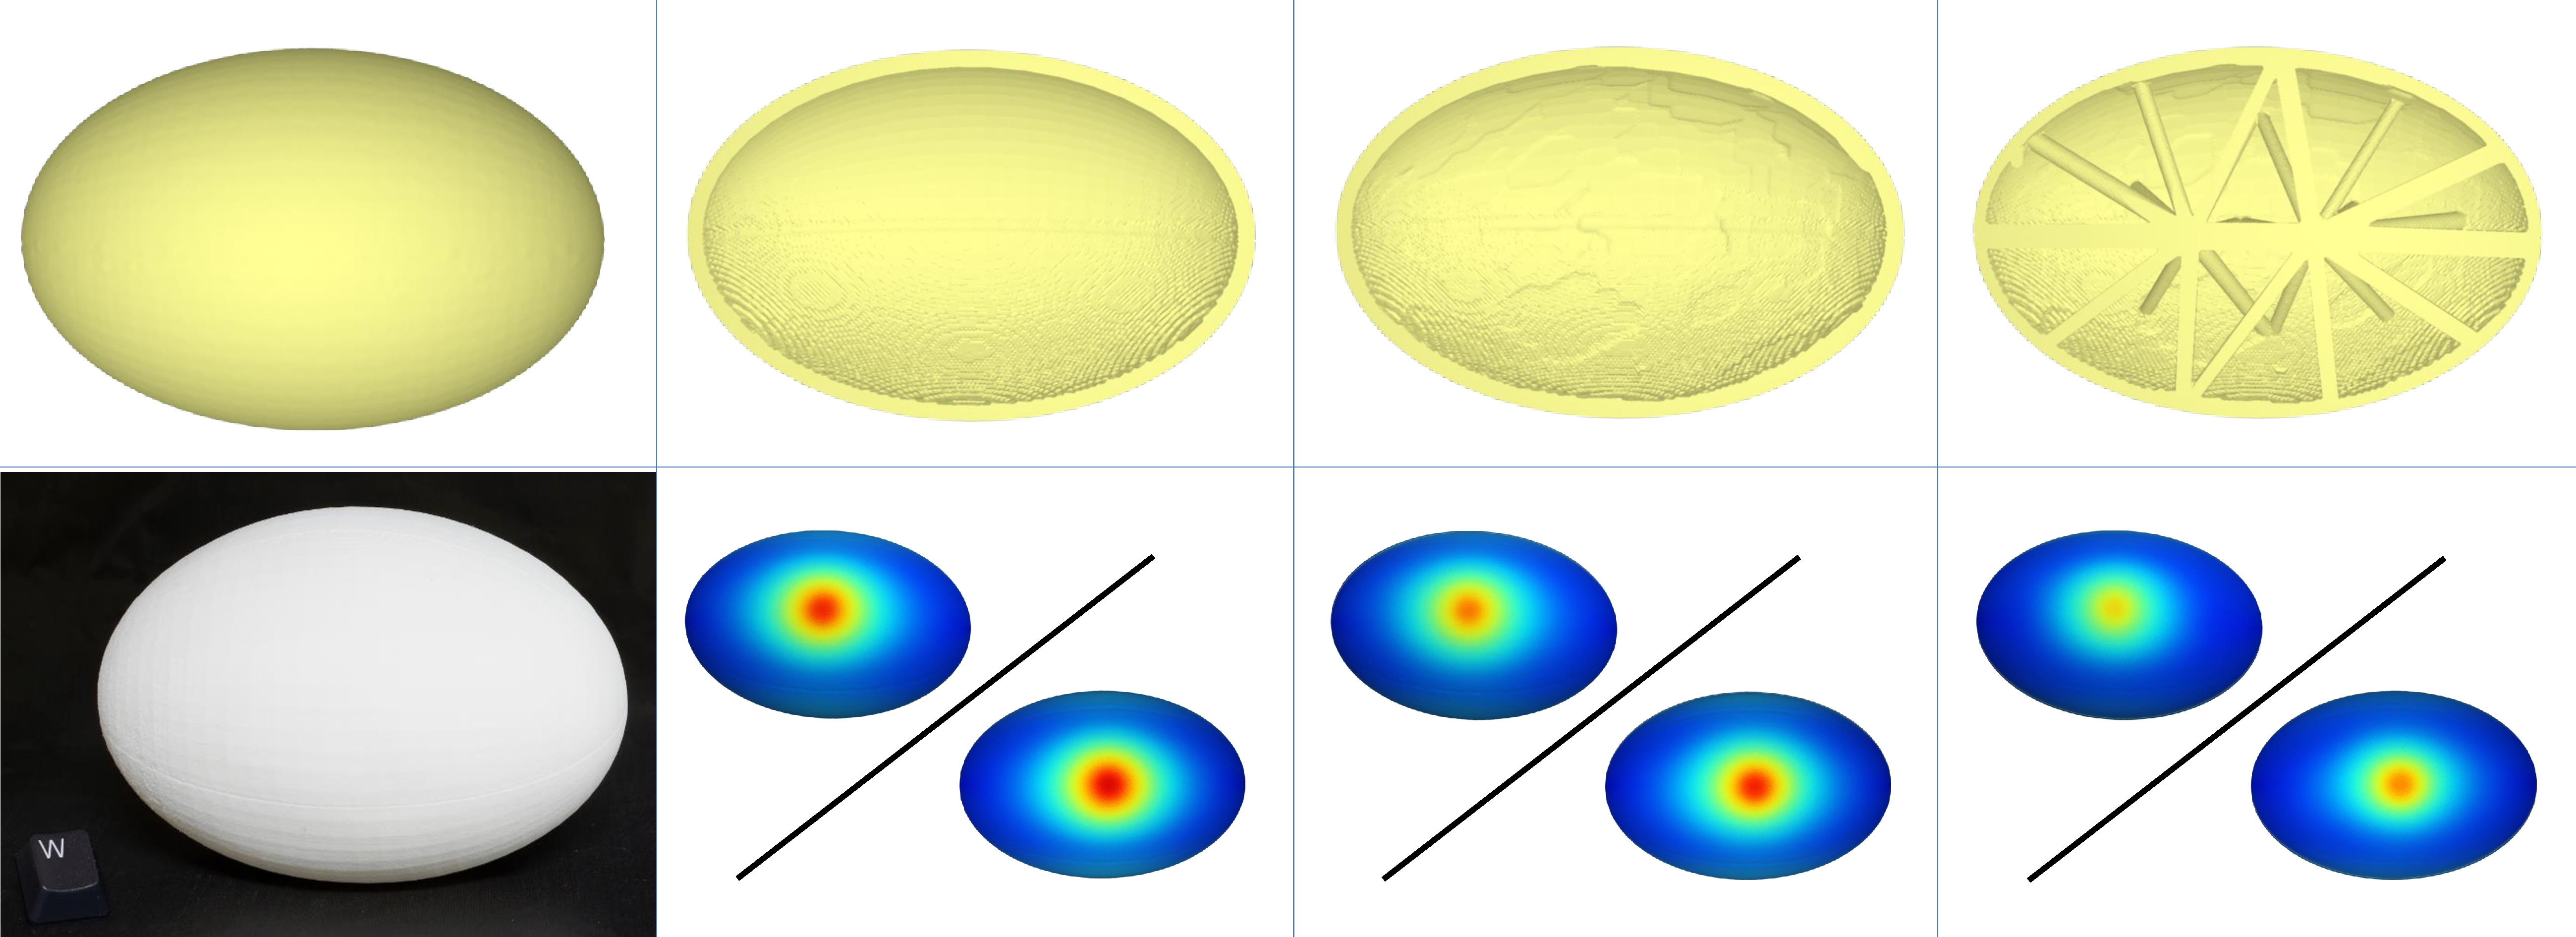
\includegraphics[width=1.0\linewidth]{Figures/football/football}
%  \centerline{
%  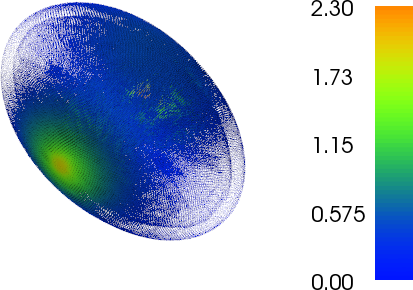
\includegraphics[width=.33\linewidth]{Figures/results/test3-cmp-hollowing-our1-disp.png}
%  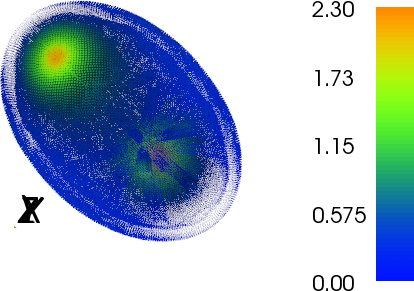
\includegraphics[width=.33\linewidth]{Figures/results/test3-cmp-hollowing-our2-disp.png}
%  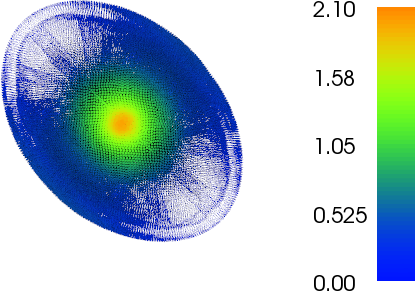
\includegraphics[width=.33\linewidth]{Figures/results/test3-cmp-hollowing-uniform1-disp.png}}
%  \vskip 0.3cm
%    \centerline{
%  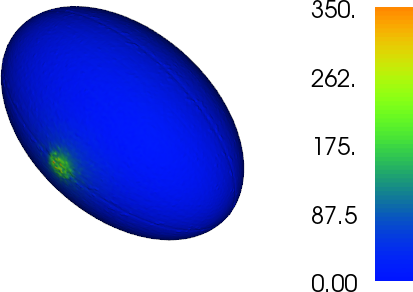
\includegraphics[width=.33\linewidth]{Figures/results/test3-cmp-hollowing-our1-stress.png}
%  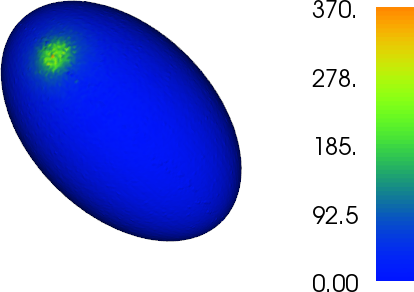
\includegraphics[width=.33\linewidth]{Figures/results/test3-cmp-hollowing-our2-stress.png}
%  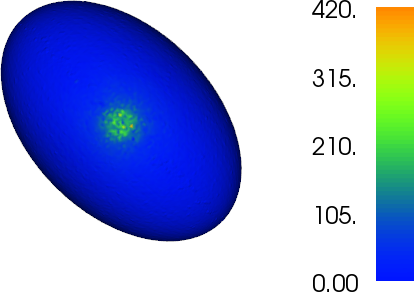
\includegraphics[width=.33\linewidth]{Figures/results/test3-cmp-hollowing-uniform1-stress.png}
%  }
  \caption{\label{fig:result-cmp-uniformhollowing}
            Comparison of our approach with uniform and adaptive hollowing methods. Left: the input mesh (top) and the printed version of our result (bottom). The top row shows the sectional view of the uniform, adaptive hollowing and our result. The bottom row shows the deformation under a pair of forces (applied on the middle). Two views are taken from the opposite direction to show the deformation on both sides. Our result gives the smallest deformation in this test.
            }
\end{figure*}


It is clear that the football model is stronger at the sharp ends and is weaker at the middle part.
Our results with inner frames suffer the least stress at the middle in these three tests shown in Figure~\ref{fig:result-cmp-uniformhollowing}.
While at the sharp ends, we have nearly the same strength as the uniform case.
We can generate stronger structures than adaptive hollowing in a straight forward manner:
i.e., looking for a solution in a larger solution space since the frames are not constrained on the surface.
Since the inner frames are sparse in this example, it is possible that our result is weaker in some regions.
For example, in large regions where no support from inner frames is available.
However, the average and variation of the stress of our results are always smaller, which verifies that our results exhibit the maximum global stiffness property.

\begin{table}[htb]
\caption{\label{tab:result-cmp-uniformhollowing}Comparison of simulation tests with hollowing methods.
         From top to bottom: statistics of uniform hollowing (uh), adaptive hollowing (ah), and our method.
         For each method, we calculate the deformation displacement (disp.) and the stress (strs.) value. The mean and var refer
         to the average and the variation, respectively.}
\centering
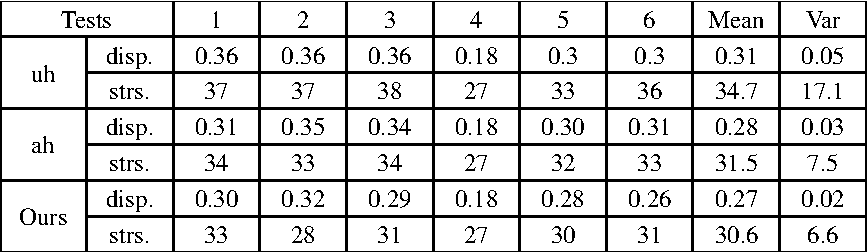
\includegraphics[width=\linewidth]{Tables/table3}
%\small
%\begin{tabular}{|c|c|c|c|c|c|c|c|c|c|}
% \hline
% tests         &               &   1  &  2   &  3   &  4   & 5     &  6    &  mean    &  var \\
% \hline \multirow{2}{*}{af}
%                    & disp.  & 0.3  & 0.32 & 0.29 & 0.18 & 0.30  &  0.31 &  0.283   &  0.027\\
%                    & strs.  & 33   & 28   & 31   & 27   & 32    &  33   &  30.67   &  6.667\\
% \hline \multirow{2}{*}{ah}
%                    & disp.  & 0.31 & 0.3  & 0.34 & 0.18 & 0.28  &  0.26 &  0.278   &  0.031\\
%                    & strs.  & 34   & 33   & 34   & 27   & 30    &  31   &  31.50   &  7.50\\
% \hline \multirow{2}{*}{uh}
%                    & disp.  & 0.36 & 0.36 & 0.36 & 0.18 & 0.3   &  0.3  &  0.31    &  0.049\\
%                    & strs.  & 37   & 37   & 38   & 27   & 33    &  36   &  34.67   &  17.0667\\
% \hline
%\end{tabular}
\end{table}


\paragraph{Comparison with cost-effective approach}
We compare the skin-frame structure of Wang et al.~\shortcite{wang:2013} in Figure~\ref{fig:result-cmp-costeffective} using the same volume of material. Since their results are optimized under a specified force distribution, our results might be weaker under this specific force. However, our structure is much stronger in almost all the other directions.

\begin{figure}[htb]
  \centering
  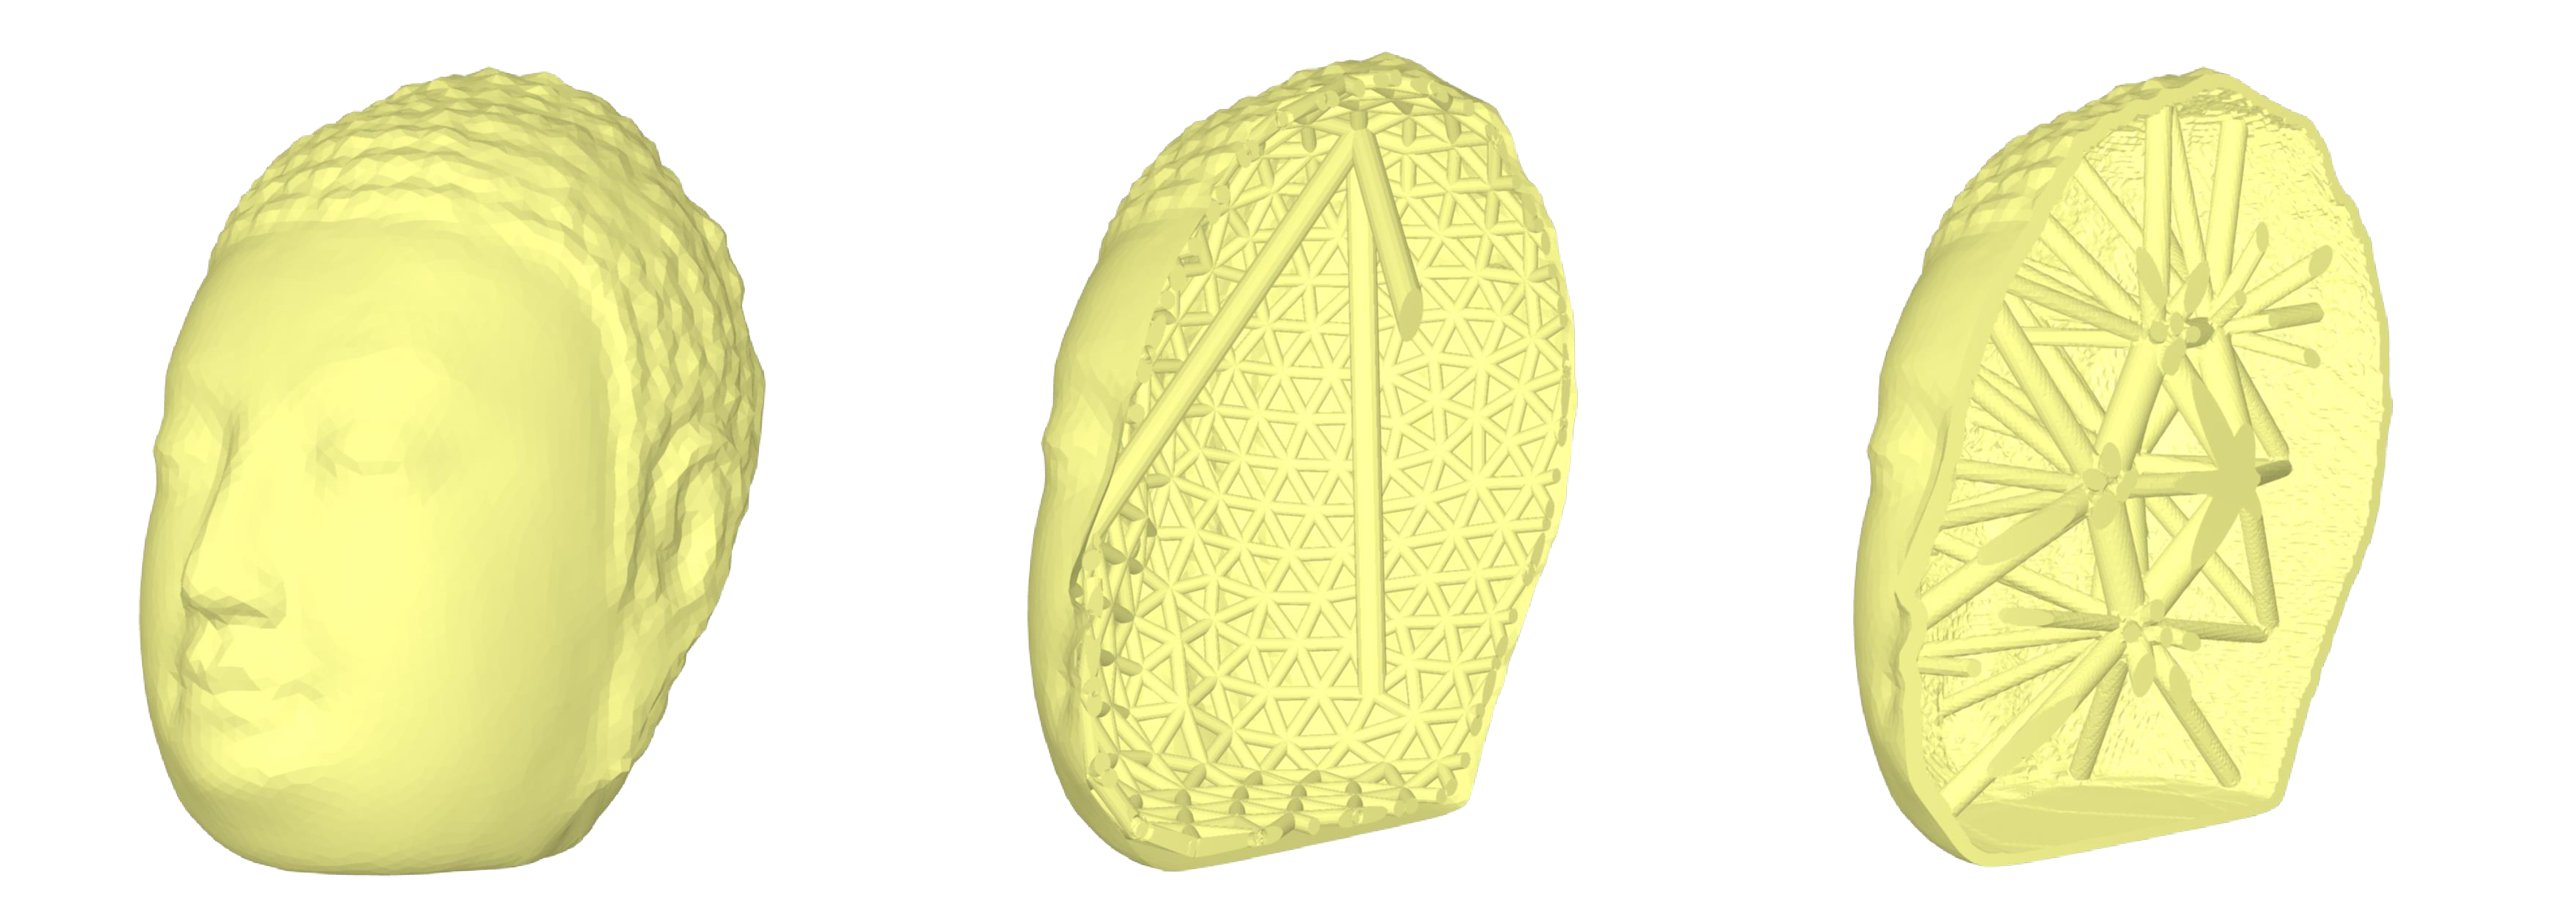
\includegraphics[width=1.0\linewidth]{Figures/head/head}
  \caption{\label{fig:result-cmp-costeffective}
  Left: the input model. Middle: the result of cost-effective method under a 40N force applied on the top of the model point to the base. Right: our result.}
\end{figure}

The cost-effective method requires a prescribed force, which provides the guides for structure optimization, but cannot fully satisfy practical usages except for very rare cases where the objects do not suffer from any other kind of force. Our experiments demonstrate that our approach is more practical for most real world objects. The statistics of performance under various force distributions used in our tests are shown in Table~\ref{tab:result-cmp-costeffective}.

\begin{table}[htb]
\caption{\label{tab:result-cmp-costeffective}
            Comparison of Wang et al.~\shortcite{wang:2013} and our method. We apply various forces for each method, where
            force 1 is applied on the top, force 2 and 3 are on the front, and force 4 and 5 are on the side of the model.
            Our result is weaker in the first case. However, the average and the variation of our method is much smaller.}
\centering
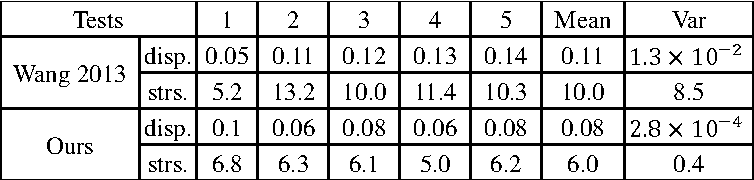
\includegraphics[width=\linewidth]{Tables/table4}
%\bigskip
%\begin{small}
%\begin{tabular}{|c|c|c|c|c|c|c|c|c|}
% \hline
% Tests           &              &   1   &   2   &   3   &   4    &  5    & mean  &  var\\ \hline
% Ours      & disp. &  0.1  & 0.06  & 0.08  &  0.06  & 0.08  & 0.076 &  2.8e-4 \\ \hline
%                 & strs.       &  6.8  &  6    &   6.1 &  5.0   &  6.2  & 6.02  &  0.4220 \\ \hline
% Wang   & disp. &  0.05 & 0.11  & 0.12  &  0.13  & 0.14  & 0.11  &  1.3e-2 \\ \hline
%                 & strs       &  5.2  & 13.0  & 9.97  &  11.4  & 10.3  & 9.97  &  8.522 \\\hline
%\end{tabular}
%\end{small}
\end{table}



